\documentclass[12pt,
               a4paper,
               article,
               oneside,
               oldfontcommands,
               norsk]{memoir}
\makeatletter
\newcommand*{\rom}[1]{\expandafter\@slowromancap\romannumeral #1@}
\makeatother
%\usepackage[utf8]{inputenc}
\usepackage{setspace}
\usepackage[T1]{fontenc}
\usepackage{titling}% the wheel somebody else kindly made for us earlier
\usepackage{fancyhdr}
\usepackage{tikz}
\usepackage{lmodern}
\usepackage{enumitem}
\usepackage{caption}
\usepackage{subcaption}
\usepackage{fancyvrb}
\usepackage[scaled]{beramono}
\usepackage[final]{microtype}
\usepackage{amssymb}
\usepackage{mathtools}
\usepackage{amsthm}
\usepackage{thmtools}
\usepackage{babel}
\usepackage{csquotes}
\usepackage{listings}
\lstset{basicstyle = \ttfamily}
\usepackage{float}
\usepackage{textcomp}
\usepackage{siunitx}
\usepackage{xcolor}
\usepackage{graphicx}
\usepackage[colorlinks, allcolors = uiolink]{hyperref}
\usepackage[noabbrev]{cleveref}
\pretolerance = 2000
\tolerance    = 6000
\hbadness     = 6000
\newcounter{probnum}[section]
\newcounter{subprobnum}[probnum] 
\usepackage{dirtytalk}
\usepackage{listings}
\usepackage{xcolor}
\usepackage{caption}
\usepackage[section]{placeins}
\usepackage{varwidth}
\definecolor{uiolink}{HTML}{0B5A9D}
\definecolor{dkgreen}{rgb}{0,0.6,0}
\definecolor{gray}{rgb}{0.5,0.5,0.5}
\definecolor{mauve}{rgb}{0.58,0,0.82}

\lstset{frame=tb,
  language=R,
  aboveskip=3mm,
  belowskip=3mm,
  showstringspaces=false,
  columns=fullflexible,
  basicstyle={\small\ttfamily},
  numbers=none,
  numberstyle=\tiny\color{gray},
  keywordstyle=\color{blue},
  commentstyle=\color{dkgreen},
  stringstyle=\color{mauve},
  breaklines=true,
  breakatwhitespace=true,
  tabsize=3
}
\usepackage{commath}
\newtheorem{theorem}{Theorem}[section]
\newtheorem{corollary}{Corollary}[theorem]
\newcommand{\Q}{ \qquad \hfill \blacksquare}
\newcommand\myeq{\stackrel{\mathclap{\normalfont{uif}}}{\sim}}
\let\oldref\ref
\renewcommand{\ref}[1]{(\oldref{#1})}
\newtheorem{lemma}[theorem]{Lemma}
\parindent 0ex
\pretitle{
	\begin{center}
		\rule[0.4pt]{300pt}{1.5pt} \\
			[0.10in]
\Huge}
		\title{STK1110}
\posttitle{\par\vskip0.3em{\scshape \textsc{ \large Obligatorisk oppgave 2}\\[-0.20in] \rule[0.4pt]{300pt}{1.5pt} \vspace{5mm}}
	\end{center}}
\author{Jonas Semprini Næss}
\begin{document}
\maketitle
NB! Kode på oppgave 1 er skrevet i samarbeid med \say{erlek@math.uio.no}
\section*{Oppgave 1:}
a.) \emph{Lag et 95 $\%$ konfidensintervall for forventet antocyaninnhold $\mu$ basert på
målingene over.} \vspace{4mm}\\ 
\textbf{Løsning:}\vspace{4mm}\\
Vi antar fra opplysningene at vi har tilnærmet normalfordelte målinger 
\begin{align*}
X_{1}, \ldots, X_{15} \sim N(\mu, \sigma)
\end{align*}
for antocyaninnhold slik at $\bar{X} \sim N(\mu, \frac{\sigma}{\sqrt{n}})$ og $Z = \frac{\bar{X} - \mu}{\sigma \backslash \sqrt{n}} \sim N(\mu, \sigma)$. Dermed vil et generelt konfidensintervall se slik ut
\begin{align*}
P(- Z_{\alpha \backslash 2} \leq \frac{\bar{X} - \mu}{\sigma \backslash \sqrt{n}} \leq Z_{\alpha \backslash 2}) &= 1 - \alpha \\[5pt]
P(- \bar{X} -Z_{\alpha \backslash 2}\frac{\sigma}{\sqrt{n}} \leq - \mu  \leq - \bar{X} + Z_{\alpha \backslash 2}\frac{\sigma}{\sqrt{n}}) &= 1 - \alpha \\[5pt]
P(\bar{X} + Z_{\alpha \backslash 2}\frac{\sigma}{\sqrt{n}} \geq  \mu  \geq \bar{X} - Z_{\alpha \backslash 2}\frac{\sigma}{\sqrt{n}}) &= 1 - \alpha \\[5pt]
\end{align*}
hvor $\alpha = 0.05$ slik at det teoretiske intervallet er gitt ved
\begin{align*}
    (\bar{X} - Z_{\alpha \backslash 2}\frac{\sigma}{\sqrt{n}}, \bar{X} + Z_{\alpha \backslash 2}\frac{\sigma}{\sqrt{n}}) \Q
\end{align*}
Ønsker vi dessuten å lage et empirisk konfidensintervall for $\mu$ tar vi simpelthen å bruker det empiriske gjennomsnittet og variansen gitt ved
\begin{align*}
    \mu &= \frac{1}{n} \sum_{i=1}^{n} X_{i} \\[5pt]
    S^2 &= \frac{1}{n-1} \sum_{i=1}^{n} \left(X_{i} - \mu \right)^2 \\[5pt]
        &= \frac{1}{n-1} \sum_{i=1}^{n} \left(X_{i} - \frac{1}{n} \sum_{i=1}^{n} X_{i} \right)^2 \\[5pt]
        &\Downarrow \\[5pt]
    S &=  \sqrt{\frac{1}{n-1} \sum_{i=1}^{n}}\left(X_{i} - \frac{1}{n} \sum_{i=1}^{n} X_{i} \right)
\end{align*}
som gir følgende konfidensintervall
\begin{align*}
    (\bar{X} - Z_{\alpha \backslash 2}\frac{S}{\sqrt{n}}, \bar{X} + Z_{\alpha \backslash 2}\frac{S}{\sqrt{n}}) \Q
\end{align*}

b.)
\emph{På Wikipedia kan vi lese at forventet antocyaninnhold i blåbær er $558$
mg/100g. Nå skal du bruke simuleringer til å late som om du måler antocyan i 15 prøver med blåbær veldig mange ganger. Generer 10000 datasett,
hvert av størrelse $n = 15$, bestående av observasjoner av de stokastiske
variablene $X_{1} \ldots X_{15} \sim N(558, 30)$. Du kan bruke rnorm()-funksjonen i R til dette. Selv om du har simulert fra en fordeling med kjent forventning og varians, skal du late som om begge disse er ukjent i det følgende. Lag et 95 $\%$ konfidensintervall for $\mu$ som i punkt a), basert på hvert av de simulerte datasettene, slik at du får 10000 intervaller. Tell opp andelen av disse intervallene som inneholder verdien 558. Kommenter og forklar}
\vspace{4mm}\\ 
\textbf{Løsning:}\vspace{4mm}\\
Som løsning av denne oppgaven vil det være fingert å enten lage en stor $N \times n$ matrise hvor $N = 10000, \ n = 15$ eller en, 1-dimensjonal array for å samle alle dataene. I det følgende R-scriptet er det benyttet en 1-d array og en enkel if-test for å sjekke hvor mange ganger $\mu = 558$ forekommer i de $10000$ forskjellige konfidensintervallene.
\begin{lstlisting}
#Oppgave 1b.
count = 0
mu_exact = 558
sd_exact = 30
iterations = 10000

for (j in 1:iterations){
  data_sett = array(1:15)
  for (i in 1:15){
    X_est = rnorm(15 ,mu_exact, sd_exact)
    data_sett[i] = X_est
  }
  mu_est = mean(data_sett)
  sd_est = sd(data_sett)
  
  con_int_low = mu_est - 1.96*sd_est/sqrt(15)
  con_int_high = mu_est + 1.96*sd_est/sqrt(15)
  if (mu_exact >= con_int_low && mu_exact <= con_int_high){
    count = count + 1
  }
}
print(count/iterations)
    \end{lstlisting}
Hvilket gir at forekomsten av $\mu = 558$ er 
\begin{verbatim}
> print(count/iterations)
[1] 0.9266.
\end{verbatim}
Altså forekommer $\mu = 558$ i rundt $93 \%$ av konfidensintervallene hvilket virker som et rimelig svar siden vi opperer med et relativt stort datasett og gjør sekvensielle beregninger av gjennomsnittet og standardavviket underveis som kan gi små avvik fra eksakte verdier for $\mu$ og $\sigma$.\vspace{4mm}\\
c.) \emph{Bruk nå i stedet det tilnærmede intervallet for store utvalg, altså}
\begin{align*}
    \left(\bar{X} - 1.96\frac{S}{\sqrt{15}},\bar{X} + 1.96\frac{S}{\sqrt{15}}  \right)
\end{align*}
\emph{med}
\begin{align*}
    \bar{X} &= \frac{1}{n} \sum_{i=1}^{n} X_{i} \\[5pt]
    S^2 &= \frac{1}{15 - 1} \sum_{i=1}^{n} \left(X_{i} - \bar{X} \right)^2 \\[5pt]
\end{align*}
\emph{og beregn dette for hvert av $10000$ datasett, generert som i b). Hvor stor andel av intervallene inneholder $\mu = 558$? Kommenter og forklar resultatet.}\vspace{4mm}\\
\textbf{Løsning:}\vspace{4mm}\\ 
I løsning av oppgaven endres det kun på estimeringsmetoden for hvert datasett slik at de numeriske tilnærmingene for $\mu$ og $\sigma$ nå må legges til. Det kan se slik ut 
\begin{lstlisting}
#Oppgave 1c.)
count = 0
mu_exact = 558
sd_exact = 30
iterations = 10000

for (j in 1:iterations){
  data_sett = array(1:15)
  mu_est = 0
  for (i in 1:15){
    X_est = rnorm(15 ,mu_exact, sd_exact)
    data_sett[i] = X_est
  }
  mu_est = sum(data_sett)/15
  sd_est = 0
  for (i in 1:15){
    sd_est = sd_est + (data_sett[i] - mu_est)^2
  }
  sd_est = sqrt(sd_est/14)
  con_int_low = mu_est - 1.96*sd_est/sqrt(15)
  con_int_high = mu_est + 1.96*sd_est/sqrt(15)
  if (mu_exact >= con_int_low && mu_exact <= con_int_high){
    count = count + 1
  }
}
print(count/iterations)
\end{lstlisting}
Hvilket gir at forekomsten av $\mu = 558$ er 
\begin{verbatim}
> print(count/iterations)
[1] 0.9287.
\end{verbatim}
Som tilsier at den empiriske tilnærmingen for $\mu$ er rimelig siden den samsvarer med resultatet for den teoretiske $\mu$ i b.) \vspace{4mm}\\ 
d.) \emph{Trekk 10000 datasett som i b) og lag et $95\%$ konfidensintervall for σ for hvert av dem. Hvor stor andel av intervallene inneholder $\sigma = 30$?}\vspace{4mm}\\
\textbf{Løsning:}\vspace{4mm}\\
For å konstruere et konfidensintervall for $\sigma$ husker vi at 
\begin{align*}
  \frac{1}{\sigma^2}\sum_{i=1}^{n} = \frac{n \hat{\sigma}^2}{\sigma^2}
\end{align*} 
hvor $\frac{n \hat{\sigma}}{\sigma^2} \sim \chi^{2}_{n}$ slik at $\hat{\sigma^2} = \frac{1}{n} \sum_{i=1}^{n} \left( X_i - \mu \right)^2$. Dermed vil et tilsvarende konfidensintervall være gitt ved
\begin{align*}
  \chi^{2}_{1 - \alpha \backslash 2}   &\leq X^{2}_{n} \leq  \chi^{2}_{\alpha \backslash 2} \\[7pt] 
  \Rightarrow \chi^{2}_{1 - \alpha \backslash 2}  &\leq \frac{n \hat{\sigma}^2}{\sigma^2} \leq  \chi^{2}_{\alpha \backslash 2} \\[7pt]
  \Rightarrow \frac{n \hat{\sigma}^2}{\chi^{2}_{1 - \alpha \backslash 2}}  &\geq \sigma^2 \geq \frac{n \hat{\sigma}^2}{\chi^{2}_{\alpha \backslash 2}} \\[7pt]
  \Rightarrow \sqrt{\frac{n \hat{\sigma}^2}{\chi^{2}_{1 - \alpha \backslash 2}}}  &\geq \sigma \geq \sqrt{\frac{n \hat{\sigma}^2}{\chi^{2}_{\alpha \backslash 2}}}\\
  &\Downarrow
\end{align*}
  $$\boxed{\left(\sqrt{\frac{n \hat{\sigma}^2}{\chi^{2}_{\alpha \backslash 2}}}, \ \sqrt{\frac{n \hat{\sigma}^2}{\chi^{2}_{1 - \alpha \backslash 2}}}  \right)}$$ \\ 
  Implementerer vi så dette resultatet kan det gi følgende løsning
\begin{lstlisting}
    #Oppgave 1d.)
    count = 0
    mu_exact = 558
    sd_exact = 30
    iterations = 10000
    
    chi2.kvant.low = qchisq(0.025,df=14)
    chi2.kvant.up = qchisq(0.975,df=14)
    
    for (j in 1:iterations){
      data_sett = array(1:15)
      mu_est = 0
      for (i in 1:15){
        X_est = rnorm(15, mu_exact, sd_exact)
        data_sett[i] = X_est
      }
      mu_est = sum(data_sett)/15
      sd_est = 0
      for (i in 1:15){
        sd_est = sd_est + (data_sett[i] - mu_est)^2
      }
    
      sd_est = sqrt(sd_est/14)
    
      low.sd=(14)*sd_est^2/chi2.kvant.up
      up.sd=(14)*sd_est^2/chi2.kvant.low
    
      cont_int_low = sqrt(low.sd)
      cont_int_high= sqrt(up.sd)
      if (sd_exact >= cont_int_low && sd_exact <= cont_int_high){
        count = count + 1
      }
    }
    
    print(count/iterations)    
\end{lstlisting}
Hvilket gir at forekomsten av $\sigma = 30$ er 
\begin{verbatim}
> print(count/iterations)
[1] 0.9503.
\end{verbatim}
Som igjen er veldig rimelig grunnet datasettet og de estimeringene vi gjør. \vspace{4mm}\\
e.) \emph{Under antakelsen om normalfordeling er $Z_{i} = \frac{X_i - \mu}{\sigma} \sim N(0,1), \ i = 1,\ldots,n$,
med $\mu = 558$ og $\sigma = 30$. Anta nå at $Z_1,\ldots, Z_{15}$ i virkeligheten er t-fordelt
med 7 frihetsgrader, altså $Z_1, \ldots, Z_{15} \myeq t_7$. Trekk nå $10000$ datasett fra denne fordelingen ved å}
\begin{enumerate}
\item Trekke $z_1 , \ldots , z_{15}$ fra $t_7$ med R-funksjonen rt().
\item La $x_i = \mu + \sigma z_i, \ i=1,\ldots,n$.
\end{enumerate}
\emph{Gjenta deretter oppgave b) med de nye datasettene. Hvor robust er metoden for å lage konfidensintervall for forventningsverdien for antakelsen om normalfordeling?}\vspace{4mm}\\ 
\textbf{Løsning:}\vspace{4mm}\\ 
Likeledes som i oppgavene over lager vi en 1-dimensjonal array på samme størrelse som tidligere. Forskjellen herfra ligger i at vi henter verdier for $Z_{i}$ fra t-fordelingen istedenfor normalfordelingen. Dermed vil en mulig løsning se slik ut 
\begin{lstlisting}
#Oppgave 1e.)

count = 0
mu_exact = 558
sd_exact = 30
iterations = 10000

for (j in 1:iterations){
  data_sett = array(1:15)
  mu_est = 0
  for (i in 1:15){
    Z_i = rt(15, 7)
    x_i = mu_exact + sd_exact*(Z_i)
    data_sett[i] = x_i
  }
  mu_est = mean(data_sett)
  sd_est = sd(data_sett)
  con_int_low = mu_est - 2.145*sd_est/sqrt(15)
  con_int_high = mu_est + 2.145*sd_est/sqrt(15)
  if (mu_exact >= con_int_low && mu_exact <= con_int_high){
       count = count + 1
     }
   }
print(count/iterations)
   
\end{lstlisting}
Hvilket gir at forekomsten av $\mu = 558$ er 
\begin{verbatim}
> print(count/iterations)
[1] 0.948.
\end{verbatim}
Dette sier oss at konfidensintervallmetoden er meget robust i henhold til antagelsen om normalfordeling fordi forekomsten $\mu = 558$ under begge analysene ligger mellom $93 \%$ og $95 \%$. \vspace{4mm}\\
f.) \emph{Trekk datasett som i e) og lag deretter $95\%$ konfidenintervall for standardavviket til $X_i$ slik som i d). Merk imidlertid at $Var(Z_i) = \frac{7}{7-2}$ slik at
variansen til $X_i$ nå er $\tilde{\sigma^2} = Var(X_i) = Var(\mu + \sigma Z_i) = \sigma^2Var(Z_i) = 1.4\sigma^2$.
Det er altså $\tilde{\sigma}$ du skal lage konfidensintervall for, og sjekke andelen intervaller som inneholder $\tilde{\sigma}$. Sammenlign med resultatene fra d) og kommenter.} \vspace{4mm}\\ 
\textbf{Løsning:}\vspace{4mm}\\ 
Prosedyren i denne oppgaven bruker både fremgangsmåten fra e.) samt konfidensintervallet fra d.). Vi husker at et $95 \%$ konfidensintervall for $\sigma$ er gitt ved 
\begin{align*}
\left( \sqrt{\frac{n \hat{\sigma}^2}{\chi^{2}_{\alpha, n}}}, \ \sqrt{\frac{n \hat{\sigma}^2}{\chi^{2}_{1- \alpha, n}}} \right)
\end{align*}
men siden vi ønsker å finne for $\tilde{\sigma} = 1.4 \sigma$ transformeres intervallet til 
\begin{align*}
  \left( \sqrt{\frac{n \hat{\sigma}^2}{1.4 \chi^{2}_{\alpha, n}}}, \ \sqrt{\frac{n \hat{\sigma}^2}{1.4 \chi^{2}_{1- \alpha, n}}} \right)
\end{align*}
hvor, som sist, $\hat{\sigma} = S$. Dette kan implementers følgelig 
\begin{lstlisting}
  #Oppgave 1f.)
  count = 0
 mu_exact = 558
 sd_exact = 30
 iterations = 10000
 chi_low = qchisq(0.025, (14), lower.tail=FALSE)
 chi_high = qchisq(0.025, (14), lower.tail=TRUE)

 for (j in 1:iterations){
   data_sett = array(1:15)
   mu_est = 0
   for (i in 1:15){
     Z_i = rt(15, 7)
     x_i = mu_exact + sd_exact*(Z_i)
     data_sett[i] = x_i
 }
   mu_est = mean(data_sett)
   sd_est = 0

   for(i in 1:15){
     sd_est = sd_est + (data_sett[i] - mu_est)^2
   }

   sd_tilde = 1.4*(sd_est/14)

   low.sd= (14)*sd_tilde/chi_low
   up.sd= (14)*sd_tilde/chi_high

   cont_int_low = sqrt((1/1.4)*low.sd)
   cont_int_high = sqrt((1/1.4)*up.sd)

   if (sd_exact >= cont_int_low && sd_exact <= cont_int_high){
        count = count + 1
      }
  }
print(count/iterations)
  \end{lstlisting}
  Hvilket gir at forekomsten av $\sigma = 30$ er 
  \begin{verbatim}
> print(count/iterations)
[1] 0.7927.
  \end{verbatim}
Her kan vi observere at modellen for konfidensintervall for $\sigma$ ved hjelp av t-fordelingsmetoden ikke er like god ei robust som for normalfordelingen ettersom forekomsten av $\sigma$ er markant lavere.
\section*{Oppgave 2:}
a.) \emph{Lag et boksplott som viser fordelingen av observasjonene. Kommenter hva du finner.} \vspace{4mm}\\
\textbf{Løsning:}\vspace{4mm}\\ 
De gitte dataene gir følgende boksplott 
\begin{lstlisting}
#Oppgave 2a.)
data <- read.table("https://www.uio.no/studier/emner/matnat/math/STK1110/data/temp.txt", 
header=T)

boxplot(data, ylab= "Kroppstemperatur", 
        main="Kroppstemperatur hos menn & kvinner") 
\end{lstlisting}
\begin{figure}[H]
	\centering
  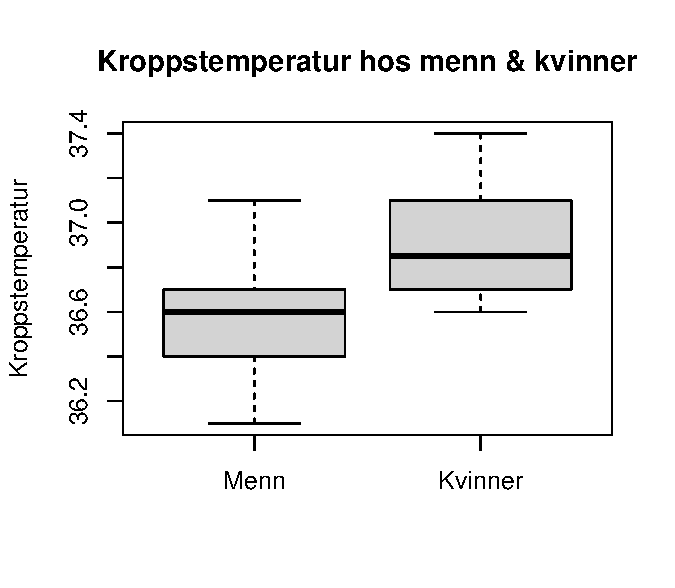
\includegraphics[scale=1.15]{Boksplott_temp.pdf}
\end{figure}
Det kan observeres fra plotet at mediantemperaturen til kvinner er noe høyere enn menns (jmf. den svarte streken på plotet), samt at de lavere verdiene for kroppstemperaturen til kvinner ligger rundt medianen til mennene. \vspace{4mm}\\ 
b.) \emph{Lag normalfordelingsplott for de to observasjonssettene, altså ett for menn og ett for kvinner. Kommenter hva du ser.}\vspace{4mm}\\ 
\textbf{Løsning:}\vspace{4mm}\\ 
For å sjekke om dataene er realiseringer av normalfordelingen kan det være beleilig å enten lage et normalsannsynlighets (Q-Q)plot eller simpelthen plotte et histogram over fordelingen med den respektive normalfordelingskurven. I løsning av oppgaven velger vi det sist nevnte. Det gir 
\begin{lstlisting}
  #Oppgave 2b.)
  hist(data$Menn, 
       freq = FALSE, 
       col="blue", 
       xlab="Temperatur i Celsius", 
       ylab="#",main="Kroppstemperatur hos menn")

curve(dnorm(x, 
      mean = mean(data$Menn), 
      sd = sd(data$Menn)),
      col = "green",
      lwd = 2,
      add = TRUE)

hist(data$Kvinner, 
    freq = FALSE, 
    col="blue", 
    xlab="Temperatur i Celsius", 
    ylab="#",main="Kroppstemperatur hos kvinner")

curve(dnorm(x, 
      mean = mean(data$Kvinner), 
      sd = sd(data$Kvinner)),
      col = "green",
      lwd = 2,
      add = TRUE)
\end{lstlisting}
\begin{figure}[H]
  \centering
  \begin{subfigure}{.5\textwidth}
    \centering
    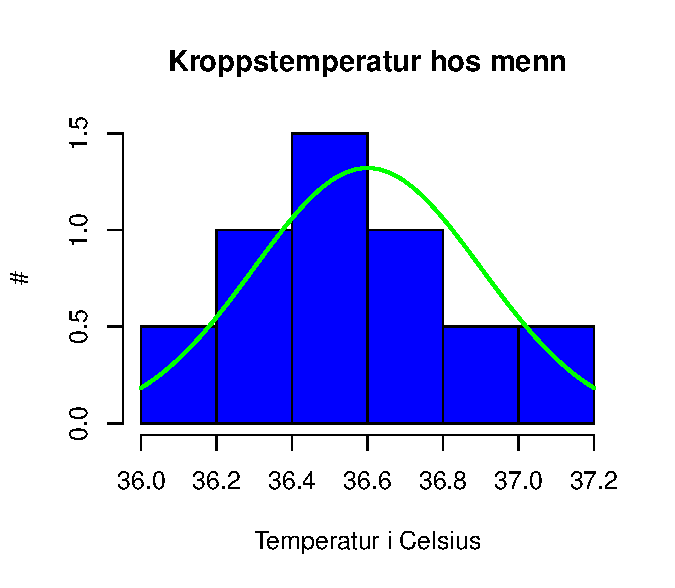
\includegraphics[width=1\linewidth]{Kropps_temp_Menn.pdf}
  \end{subfigure}%
  \begin{subfigure}{.5\textwidth}
    \centering
    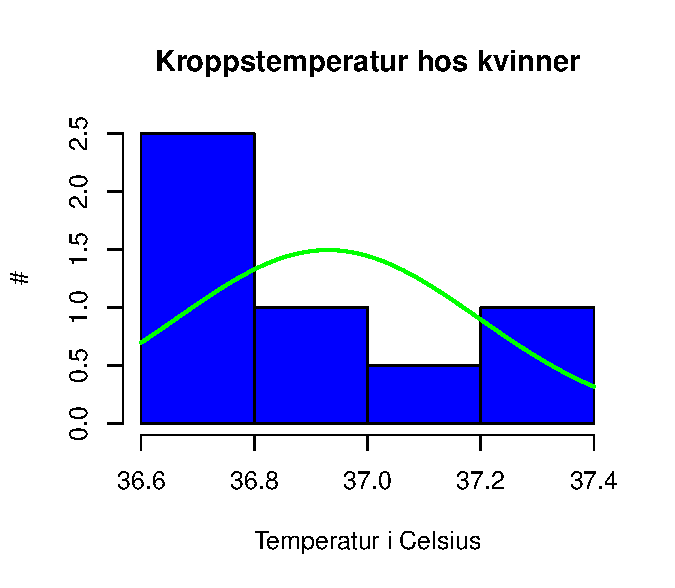
\includegraphics[width=1\linewidth]{Kropps_temp_Kvinner.pdf}
  \end{subfigure}
  \caption{Histogram og normalplott av dataene}
  \end{figure}
Hvor vi observerer fra plottene at hverken dataene for menn eller kvinner er eksakt normalfordelte, men at antagelsen om normalfordeling hos menn er betraktelig bedre enn hos kvinner (jmf. jevnere haler og hovedvekten av dataene faller inn under gjennomsnittet). \vspace{4mm}\\ 
c.) \emph{Anta at variansen er den samme for de to utvalgene, og test med signifikansnivå $5\%$ om det er noen forskjell i forventet kroppstemperatur. Beregn P-verdien, og lag et $95\%$ konfidensintervall for denne forskjellen.} \vspace{4mm}\\ 
\textbf{Løsning:}\vspace{4mm}\\ 
For å løse oppgaven er det fornuftig å benytte seg av hypotesetesting for å sjekke om det er rimelig å anta at det forskjellig forventet kroppstemperatur mellom kvinner og menn. Dermed har vi hypotesene 
\begin{align*}
  H_{0} : \mu_{k} - \mu_{m} &= 0 \\[5pt]
  H_{a} : \mu_{k} - \mu_{m} &\neq 0 \\[5pt].
\end{align*}
Siden vi antar normalfordeling på dataene benytter vi oss av en two sample T-test, gitt ved 
\begin{align*}
  T = \frac{\bar{X} - \bar{Y} - \left(\mu_{k} - \mu_{m}\right)}{\sqrt{S_{p}^{2} \left(\frac{1}{m} + \frac{1}{n}\right)}}.
\end{align*}
Hvor, i vårt tilfelle $m = n$ siden utvalgsstørrelsen er like store. Videre er $S_{p}^{2}$ gitt ved 
\begin{align*}
  S_{p}^{2} &= \frac{m-1}{m +n - 2}S_{1}^2 +  \frac{m-1}{m +n - 2}S_{2}^2 \\[5pt] 
            &= \frac{m-1}{2m - 2}\left(S_{1}^{2} + {S_{2}^2} \right) \\[5pt]
            &= \frac{1}{2}S_{1}^{2} +\frac{1}{2}S_{2}^{2}
\end{align*}
hvor vi vet at $S_{1}^{2}, S_{2}^2$ er utvalgsvariansen til de respektive dataene. Herfra bruker vi R til å teste for tilfelle hvor $H_{0}$ er antatt riktig.
\begin{lstlisting}
#Oppgave 2c.)

m = 10

SP = ((m-1)/(2*m-2))*(var(data$Kvinner)+var(data$Menn))

Tvalue = (mean(data$Kvinner)-mean(data$Menn))/(sqrt(SP*(2/m)))

print(round(c(SP, Tvalue), 4))
\end{lstlisting}
som gir verdiene 
\begin{verbatim}
> print(round(c(SP, Tvalue), 4))
[1] 0.0812 2.5901.
\end{verbatim}
Siden variansen er antatt lik for de utvalgene kan vi nå finne den kritiske $t$-verdien med $\alpha = 0.05$ og frihetsgrader 
\begin{align*}
 \nu &= \frac{\left(\frac{S_{1}^{2}}{m} + \frac{S_{2}^2}{n} \right)^2}{\frac{\left(S_{1}^2 \backslash m \right)^2}{m-1} + {\frac{\left(S_{2}^2 \backslash n \right)^2}{n-1}}} \\[7pt] 
 &= \frac{\left(2 \frac{S^2}{m} \right)^2}{\frac{2\left( S^2 \backslash m \right)^2}{m-1}}, \qquad \boxed{S^{2} = S_{1}^2 + S_{2}^2} \\[7pt] 
 &= \frac{4}{\frac{2}{m-1}} = 2(m-1) = 18.
\end{align*}
Bruker vi så t-tabellen gir det 
\begin{align*}
  t_{\text{crit}} = t_{\alpha \backslash 2, 18} = 2.1009.
\end{align*}
For å kunne avvise nullhypotesen med $95 \%$ sikkerhet ($\alpha = 0.05$) må følgende likning være oppfylt 
\begin{align*}
  |t_{\text{crit}}| &\leq T \\[5pt] 
  2.1009 &\leq 2.5901.
\end{align*}
Dette er grunnet at differansen mellom $T$ og $0$ (vår nullhypotese) er større enn $t_{\text{crit}}$. Sluttvis ønsker vi å finne $P$-verdien og konstruere et $95 \%$ konfidensintervall for forskjellen i forventet kroppstemperatur. $P$-verdien til utvalgene korresponderer til sanmsynligheten for at nullhypotesen er sann gitt en signifikansverdi. Altså vil nullhypotesen påstås sann dersom $P$-verdien er større enn $\alpha$. \vspace{2mm}\\
Vi har at generelle $P$-verdier er lik arealet til venstre og høyre for $T$-kurven. Altså 
\begin{align*}
  P_{\text{Verdi}} = P(-2.59 \leq T \leq 2.59)
\end{align*}
og siden $T$-kurven i dette tilfellet er symmetrisk om midtpunktet vil arealet på venstre og høyresiden være like. Dermed kan vi skrive $P$-verdien som 
\begin{align*}
  P_{\text{Verdi}} = 2P(T \leq 2.59)
\end{align*}
Herfra kan vi simulere løsning ved hjelp av R 
\begin{lstlisting}
  pvalue = 2*pt(Tvalue, df=18, lower.tail = F)
\end{lstlisting}
\begin{verbatim}
> print(pvalue)
[1] 0.01848131
\end{verbatim}
hvor vi observerer at $P_{\text{Verdi}} \leq \alpha$ som betyr at vi kan avvise nullhypotesen med $95 \%$ sikkerhet. Herfra skal vi konstruere et $95 \%$ konfidensintervall for forksjellen i forventet kroppstemperatur, med $\alpha = 0.05$. For en vilkårlig pooled t-test gir det 
\begin{align*}
  \left( \bar{X} - \bar{Y} \right) \pm t_{\alpha \backslash 2, \nu} \sqrt{\frac{S_{1}^2}{m} + \frac{S_{2}^2}{n}}
\end{align*}
hvor $m = n = 10$ og $\nu = 18$. Løser vi med R får vi 
\begin{lstlisting}
  CF = qt(0.025, 18, lower.tail = FALSE)
  error = CF*sqrt((var(data$Kvinner) + var(data$Menn))/10)
  diff = mean(data$Kvinner)-mean(data$Menn)
  leftside <- diff - error
  rightside <- diff + error
  print(c(leftside, rightside))
\end{lstlisting}
\begin{verbatim}
> print(c(leftside, rightside))
[1] 0.06232131 0.59767869
\end{verbatim}
og dermed kan vi være $95 \%$ sikkre på at 
\begin{align*}
  0.06232131 \leq \bar{X} - \bar{Y} \leq 0.59767869.
\end{align*}
Kan tilleggsvis sjekke med t.test() i R at alt vi har beregnet er korrekt.
\begin{lstlisting}
  t.test(x = data$Kvinner, 
         y=data$Menn, 
         mu = 0, 
         paired = FALSE, 
         var.equal = TRUE, 
         conf.level = 0.95)
\end{lstlisting}
\begin{verbatim}
Two Sample t-test

data:  data$Kvinner and data$Menn
t = 2.5901, df = 18, p-value = 0.01848

alternative hypothesis: true difference in means is not equal to 0
95 percent confidence interval:

 0.06232131 0.59767869

sample estimates:
mean of x mean of y 
    36.93     36.60 
\end{verbatim}
d.) \emph{Gjennomfør testen og beregn P-verdien også i det tilfellet der en ikke antar felles varians. Diskuter og forklar resultatene.}\vspace{4mm}\\ 
\textbf{Løsning:}\vspace{4mm}\\ 
Når man ikke antar felles varians må vi beregne de nye frihetsgradene gitt ved  
\begin{align*}
\nu &= \frac{\left(\frac{S_{1}^{2}}{m} + \frac{S_{2}^2}{n} \right)^2}{\frac{\left(S_{1}^2 \backslash m \right)^2}{m-1} + {\frac{\left(S_{2}^2 \backslash n \right)^2}{n-1}}} \\[7pt] 
 &= \frac{\left(\frac{S_{1}^2 + S_{2}^2}{m} \right)^2}{\frac{\frac{S_{1}^4 + S_{2}^4}{m^2}}{m-1}}.
\end{align*}
$T$ verdien er den samme som i oppgave c.), og følgende R script kan lages 
\begin{lstlisting}
  v = ((var(data$Menn) +var(data$Kvinner))/m)^2/(((var(data$Menn)^2 + var(data$Kvinner)^2)/(10^2))/(9))

  pvalue2 = 2*pt(Tvalue, df=v, lower.tail = F)

  CF2 = qt(0.025, v, lower.tail = FALSE)

  error2 = CF2*sqrt((var(data$Kvinner) + var(data$Menn))/m)

  diff = mean(data$Kvinner)-mean(data$Menn)

  l2<- diff - error2
  r2 <- diff + error2
\end{lstlisting}
\begin{verbatim}
> print(pvalue2)
[1] 0.01863038
> print(c(l2, r2))
[1] 0.06203301 0.59796699
\end{verbatim}
Sjekker så om dette stemmer overens med t.test()
\begin{lstlisting}
  t.test(x = data$Kvinner, y=data$Menn, mu = 0, paired = FALSE, var.equal = FALSE, conf.level = 0.95)
\end{lstlisting}
\begin{verbatim}
  Welch Two Sample t-test

  data:  data$Kvinner and data$Menn
  t = 2.5901, df = 17.734, p-value = 0.01863

  alternative hypothesis: true difference in means is not equal to 0
  95 percent confidence interval:

  0.06203301 0.59796699
  sample estimates:
  mean of x mean of y 
      36.93     36.60 
\end{verbatim}
hvor vi observerer at verdiene stemmer godt overens selv om testen runder av frihetsgraden til tre desimaler og man således kan få små avrundingsfeil. En kan også observere at nullhypotesen kan forkastes i dette tilfellet også. \vspace{4mm}\\ 
e.) \emph{Utled og gjennomfør en F-test for å sjekke om det er noen grunn til å påstå at variansene er forskjellige. Sjekk mot var.test() i R .}\vspace{4mm}\\ 
\textbf{Løsning:}\vspace{4mm}\\ 
I denne oppgaven skal vi sjekke om vi med pålitelig grunnlag kan påstå om variansene er forskjellige. Dette gjør vi ved hjelp av en F-test. Observatoren til F-testen er da gitt ved 
\begin{align*}
  F = \frac{S_{1}^2 \backslash \sigma_{1}^{2}}{S_{2}^2 \backslash\sigma_{2}^{2}}
\end{align*}
der 
\begin{align*}
  \nu_{1} = m - 1, \ \nu_{2} = n-1.
\end{align*}
Konstruerer så hypotesen
\begin{align*}
  H_{0}: \sigma_{1}^{2} = \sigma_{2}^{2} \\[5pt]
  H_{a}: \sigma_{1}^{2} \neq \sigma_{2}^{2} \\[5pt]
\end{align*}
hvor vi observerer at nullhypotesen vil anta at forholdet mellom $S_{1}^2$ og $S_{2}^2$ er 1. Altså kan vi skrive 
\begin{align*}
  f = \frac{S_{1}^2}{S_{2}^2} \sim f_{m-1, n-1}.
\end{align*}
Setter vi så inn for verdien til variansen for begge kjønn gir det 
\begin{align*}
  f = 1.279.
\end{align*}
Dermed kan vi ved en two-tailed test avvise nullhypotesen dersom 
\begin{align*}
  f \geq F_{\alpha \backslash 2, m - 1, n -1}
\end{align*}
som ved hjelp av R gir oss 
\begin{lstlisting}
  Fratio = var(data$Menn)/var(data$Kvinner)
  alpha = 0.05
  fcrit = qf(alpha/2,9,9, lower.tail = F)
\end{lstlisting}
hvor, ettersom vi benytter oss av den største variansen bruker en right-tailed test, som gir verdiene
\begin{verbatim} 
> print(c(Fratio, fcrit))
[1] 1.279251 4.025994.
\end{verbatim}
Her er det åpenbart at $|f_{\text{crit}}| > F$ som betyr at vi ikke kan avvise nullhypotesen, og den korresponderende P-verdien er 
\begin{align*}
  P_{\text{Verdi}} = 2P(F \geq f_{\text{crit}})
\end{align*}
som ved hjelp av R gir 
\begin{lstlisting}
  Fratio = var(data$Menn)/var(data$Kvinner)

  PvalueF = 2*pf(Fratio, df1=9, df2=9, lower.tail = F)
\end{lstlisting}
\begin{verbatim} 
> print(PvalueF)
[1] 0.7196901.
\end{verbatim}
Sjekker sluttvis resultatene opp mot var.test() funksjonen
\begin{lstlisting}
var.test(data$Menn, data$Kvinner)
\end{lstlisting}
\begin{verbatim} 
  F test to compare two variances

  data:  data$Menn and data$Kvinner

  F = 1.2793, num df = 9, denom df = 9, p-value = 0.7197
  alternative hypothesis: true ratio of variances is not equal to 1
  
  95 percent confidence interval:
   0.3177479 5.1502577

  sample estimates:
  ratio of variances 
            1.279251 
\end{verbatim}
som viser at verdiene våre stemmer overens med de fra testen.\vspace{4mm}\\
f.) \emph{Se nå på situasjonen der en vurderer å innhente to nye målinger. La $X_{11}$ være verdien for kvinnen og $Y_{11}$ verdien for mannen, slik at forskjellen er $X_{11} − Y_{11}$. Vi antar nå at alle observasjonene er normalfordelte med samme varians. Begrunn at et rimelig anslag for $X_{1}1 − Y_{11}$ er differansen mellom gjennomsnittet av de 10 eksisterende målingene for kvinner og menn, altså $\bar{X}- \bar{Y}$. Hva er fordelingen til $X_{11} − Y_{11}-(\bar{X} - \bar{Y})$? Bruk dette til å lage et $95\%$ prediksjonsintervall for $X_{11} − Y_{11}$, altså et intervall som med sannsynlighet $0.95$ inneholder $X_{11} − Y_{11}$. Dette er gjennomgått for ett-utvalgs-situasjonen på forelesning. Forklar hva som er forskjellen mellom et slikt intervall og et konfidensintervall for $\mu_{1} − \mu_{2}$ . Hvordan skal et prediksjonsintervall tolkes? [Hint: Siden alle variablene er normalfordelte, er $X_{11} − Y_{11}-(\bar{X} - \bar{Y})$ også det. Det er derfor nok å beregne forventning og varians for å finne fordelingen til denne størrelsen.]}\vspace{4mm}\\ 
\textbf{Løsning:}\vspace{4mm}\\ 
Vi antar at variansen mellom menn og kvinner lik og vi ønsker å lage et prediksjonsintervall for forskjellen $X_{11} - Y_{11}$. Det gir at $E[X_{11} - Y_{11}] = \mu_{X} - \mu_{Y}$ med respektive estimator $\tilde{X}_n - \tilde{Y}_n$ for utvalgsmengden $m = n = 10$. Siden vi har antatt at datamengden er realiseringer av normalfordelingen vil likeledes en linjærkombinasjon av stokatiske variable $X, Y \sim N(\mu, \sigma)$ og gjennomsnittene deres $\bar{X}, \bar{Y} \sim N(\mu, \sigma)$ være normalfordelte. 
Altså er $X_{11} − Y_{11}-(\bar{X} - \bar{Y}) \sim N(\mu, \sigma)$.
\section*{Oppgave 3:}
a.) \emph{ Er forskjellen mellom mødre og fedre signifikant? Formuler hypoteser, beregn en p-verdi, og konkluder. Kommenter kort.}\vspace{4mm}\\ 
\textbf{Løsning:}\vspace{4mm}\\ 
Det er rimelig å anta at vi arbeider med en binomisk problemstilling ettersom oppgaveteksten er formulert i en \say{ja, nei} form eller $P, \bar{P}$. Dermed kan vi si at fedre som svarer ja er representert ved 
\begin{align*}
  X \sim \text{Bin}(3000, 0.162)
\end{align*}
hvor $n = 3000$ og $p = 0.162$.På samme måte for mødre er 
\begin{align*}
  Y \sim \text{Bin}(3000, 0.147).
\end{align*}
For å sjekke om det er en signifikant forskjell mellom mødre og fedre kan vi konstruere følgende hypotese 
\begin{align*}
  H_{0}: p_{1} - p_{2} = 0 \\[5pt] 
  H_{a}: p_{1} - p_{2} \neq 0.
\end{align*}
Hvor $p_{1}, p_{2}$ svarer til de respektive sannsynlighetene for at en person fra hvert kjønn svarer ja. Videre har vi også estimatorene $\hat{p_{1}}, \hat{p_{2}}$
\begin{align*}
\hat{p_{1}} = \frac{X}{n}, \ \hat{p_{2}} = \frac{Y}{m}
\end{align*}
for $p_{1},p_{2}$ som er forventingsrette 
\begin{align*}
  E\left(\hat{p_{1}} - \hat{p_{2}} \right) &= E\left( \frac{X}{n} - \frac{Y}{m} \right) \\[7pt]
  &= \frac{1}{n}np_{1} - \frac{1}{m}mp_{2} \\[7pt]
  &= p_{1} - p_{2}
\end{align*}
og man kan dermed skrive Z-funksjonen (scoren) som 
\begin{align*}
  Z = \frac{\hat{p_{1}} - \hat{p_{2}} - E \left( \hat{p_{1}} - \hat{p_{2}}\right)}{\text{SD}(\hat{p_{1}} - \hat{p_{2}})}.
\end{align*}
Variansen til $\hat{p_{1}} - \hat{p_{2}}$ er gitt ved
\begin{align*}
  \text{Var}(\hat{p_{1}} - \hat{p_{2}}) &= \text{Var}\left(\frac{X}{n} \right) + \text{Var}\left(\frac{Y}{m} \right), \qquad \boxed{\text{Var(-Y) = Var(Y)}} \\[7pt] 
  &= \frac{1}{n^2}np_{1}(1 - p_{1}) + \frac{1}{m^2}mp_{2}(1 - p_{2}) \\[7pt]
  &= \frac{p_{1}(1 - p_{1})}{n} + \frac{p_{2}(1 - p_{2})}{m}
\end{align*}
og siden nullhypotesen antar $p_{1} - p_{2} = 0$ gir det sluttvis 
\begin{align*}
  Z = \frac{\hat{p_{1}} - \hat{p_{2}} - E \left( \hat{p_{1}} - \hat{p_{2}}\right)}{\sqrt{\frac{p_{1}(1 - p_{1})}{n} + \frac{p_{2}(1 - p_{2})}{m}}}.
\end{align*}
Bruker vi forutsetningen for nullhypotesen ser vi at $p_{1} = p_{2} = p$, og siden $n = m$ omskrives nevneren til 
\begin{align*}
\sqrt{\frac{2p(1-p)}{n}}.
\end{align*}
Men siden $p$ er ukjent må den approksimeres ved 
\begin{align*}
  \hat{p} = \frac{1}{2} \left(\hat{p}_{1} + \hat{p}_{2} \right).
\end{align*}
Finurlig nok er som nevnt utavlgsmengdene like store som betyr at de \say{veier} like mye og da holder det å kun ta gjennomsnittet av de. Det gir 
\begin{align*}
  \hat{p} = \frac{1}{2} \left(0.162 + 0.147 \right) = 0.1545
\end{align*}
Bruker vi R for å løse siste del har vi 
\begin{lstlisting}
#Oppgave 3a.)
N = 3000 X = 486
Y = 441
p1 = X/N
p2 = Y/N
phat = (1/2)*(p1 + p2)
qhat = (1 - phat)
Z = (p1-p2)/(sqrt(phat*qhat*(2/N)))
  \end{lstlisting}
  \begin{verbatim} 
>print(Z)
[1] 1.60737 
  \end{verbatim}
og tilslutt sjekker vi P-verdien for å bestemme om vi skal forkaste nullhypotesen eller ei 
\begin{align*}
  P_{\text{Verdi}} = 2P(Z \leq 1.60737)
\end{align*}
som igjen ved hjelp av R gir 
\begin{lstlisting}
  #Oppgave 3a.)
  pvalue = 2*pt(Z, df=5998, lower.tail = F)
\end{lstlisting}
\begin{verbatim} 
> pvalueopg3
[1] 0.1080259
\end{verbatim}
og vi kan konkludere med at vi kan forkaste nullhypotesen dersom signifikansverdien er høyere enn $0.108$ eller mer presist at $\alpha = 0.1 \ \lor \ \alpha < 0.1$. \vspace{4mm}\\ 
b.) \emph{Kontroller svaret ditt ved å bruke prop.test() i R.}\vspace{4mm}\\ 
\textbf{Løsning:}\vspace{4mm}\\
Bruker prop.test() i R og får 
\begin{lstlisting}
  #Oppgave 3b.)
  prop.test( x = c(486,441) , 
            n = c(3000, 3000), 
            alternative = "two.sided", 
            correct = FALSE)
\end{lstlisting}
\begin{verbatim} 
2-sample test for equality of proportions without continuity correction
              data:  
c(486, 441) out of c(3000, 3000)

X-squared = 2.5836, df = 1, p-value = 0.108

alternative hypothesis: two.sided
95 percent confidence interval:
 -0.003286474  0.033286474
sample estimates:
prop 1 prop 2
0.162 0.147
\end{verbatim}
Hvor vi observerer at P-verdien stemmer overens med det vi fikk i a.) 
\begin{align*}
  \int_{a}^{b} f(x) \ dx = G(\gamma) - F(\alpha)
\end{align*}
\end{document}